\documentclass[]{beamer}

%Package declarations
\usepackage[utf8]{inputenc}
\usepackage[spanish]{babel}
\usepackage{natbib}
\usepackage{graphicx}

%Theme related configurations
\usecolortheme{seahorse}
\usetheme{Berkeley}

% \graphicspath{..\Docs}



%Title of the presentation
\title{Instrumentación electrónica avanzada cómo oportunidad para la automatización de sistemas de producción de alimentos en áreas del corredor seco.}
\author{Luis Guillermo García Ordóñez}
\date{10 de Noviembre 2018}



\begin{document}
\maketitle

\begin{frame}{¿Qué es el corredor seco?}

\note{Desde un punto de vista ecológico}
Es una zona de bosque tropical seco que presenta un patrón de lluvias irregulares, caracterizado por extensos períodos de sequías reduciéndose hasta 30\% y 40\% durante el período del niño.
\begin{figure}
    \centering
    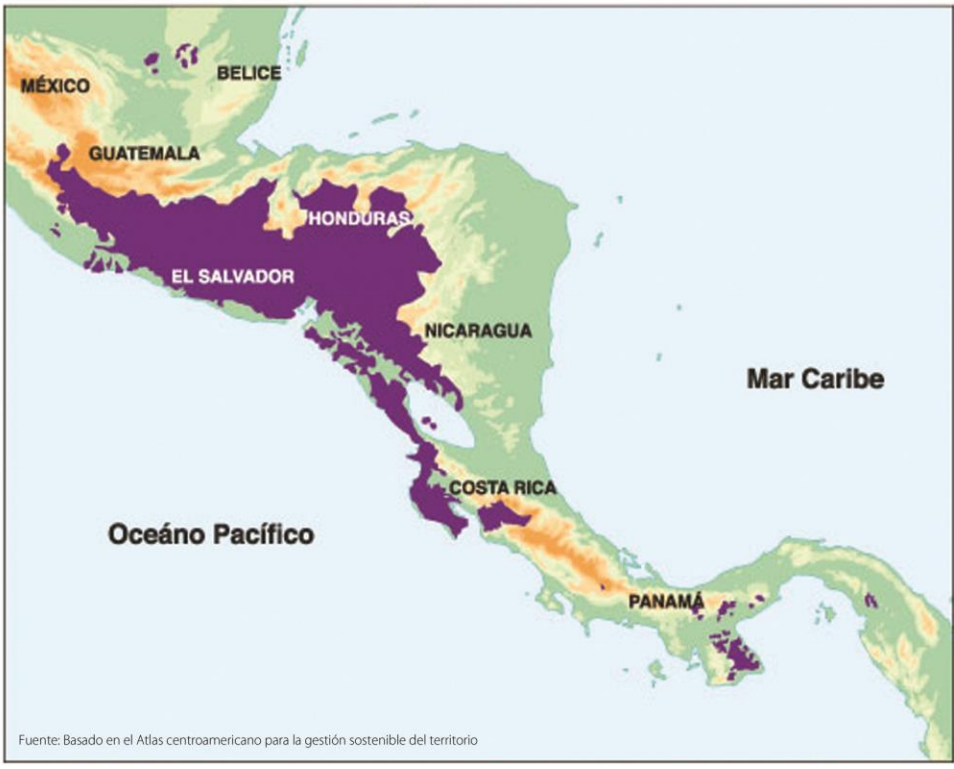
\includegraphics[width=0.5\textwidth]{Docs/Mapa_CS}
    \caption{\small \textit{Dry Corridor Central America}, Situation Report, June 2016, \textbf{FAO}}
    \label{fig:my_label}
\end{figure}
\end{frame}

\begin{frame}{}
\begin{figure}
    \centering
    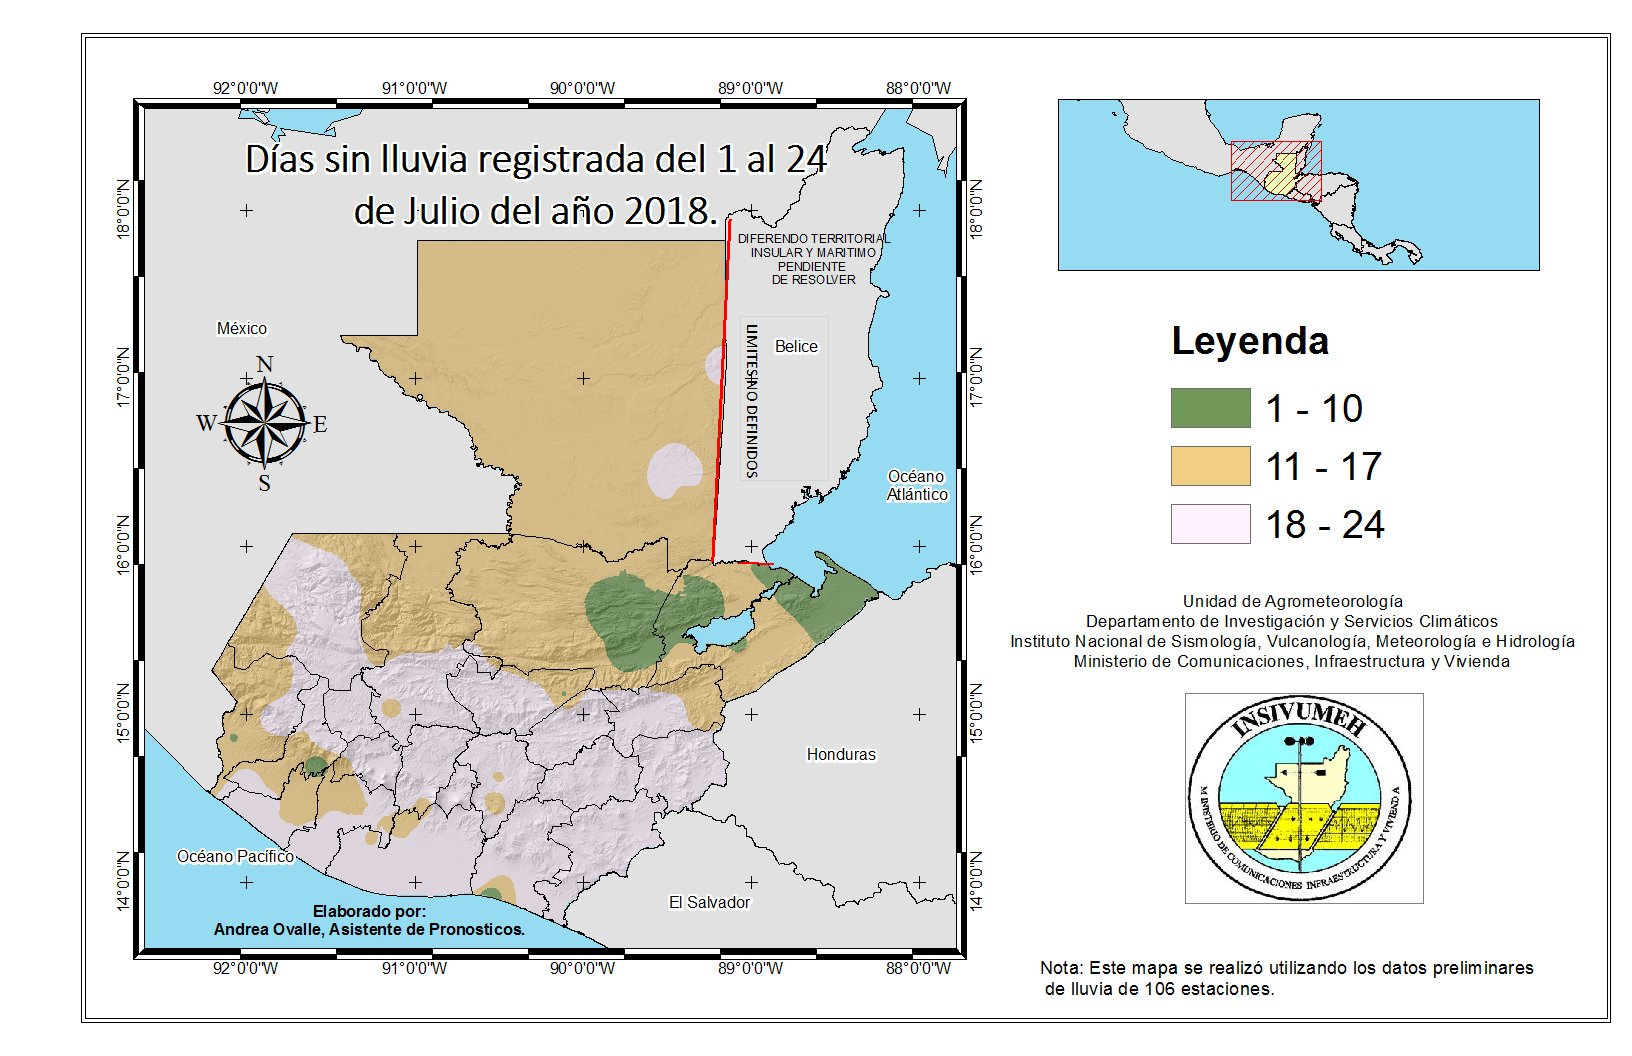
\includegraphics[width=0.9\textwidth]{Docs/diassinlluvia}
    % \caption{Caption}
    \label{fig:my_label}
\end{figure}
\end{frame}

\begin{frame}{En números}
    \begin{figure}
        \centering
        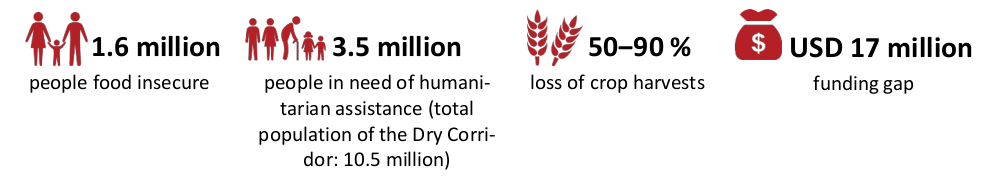
\includegraphics[width=0.8\textwidth]{Docs/cs_in_numbers}
        \caption{Cífras estimadas en centroamérica;  FAO, \textit{Situation Report}, Junio 2016}
        \label{fig:my_label}
    \end{figure}
    \begin{itemize}
      \item Durante la época de lluvias, la primera temporada de producción de maíz y frijol contribuye en 60 y 35 porciento, respectivamente, a la producción total anual.
      \item 1.5 millones de personas necesitan ayuda humanitaria en el 2016. %FAO Situation Report 2016
      \item 175,126 hectáreas de cultivo (maíz, frijol) perdídas en el 2018. %FAO GIEWS UPDATE
      \item 1,290,785 Personas afectadas en Guatemala. %FAO GIEWS UPDATE
    \end{itemize}
\end{frame}


\end{document}
